\documentclass{article}


% if you need to pass options to natbib, use, e.g.:
%     \PassOptionsToPackage{numbers, compress}{natbib}
% before loading neurips_2023


% ready for submission
\usepackage[final]{neurips_2023}


% to compile a preprint version, e.g., for submission to arXiv, add add the
% [preprint] option:
%     \usepackage[preprint]{neurips_2023}


% to compile a camera-ready version, add the [final] option, e.g.:
%     \usepackage[final]{neurips_2023}


% to avoid loading the natbib package, add option nonatbib:
%    \usepackage[nonatbib]{neurips_2023}


\usepackage[utf8]{inputenc} % allow utf-8 input
\usepackage[T1]{fontenc}    % use 8-bit T1 fonts
\usepackage{hyperref}       % hyperlinks
\usepackage{url}            % simple URL typesetting
\usepackage{booktabs}       % professional-quality tables
\usepackage{amsfonts}       % blackboard math symbols
\usepackage{nicefrac}       % compact symbols for 1/2, etc.
\usepackage{microtype}      % microtypography
\usepackage{xcolor}         % colors
\usepackage{graphicx}

\graphicspath{ {./images/} }


\title{Comparative Analysis of Intrusion Detection Models on the NSL-KDD Dataset}


% The \author macro works with any number of authors. There are two commands
% used to separate the names and addresses of multiple authors: \And and \AND.
%
% Using \And between authors leaves it to LaTeX to determine where to break the
% lines. Using \AND forces a line break at that point. So, if LaTeX puts 3 of 4
% authors names on the first line, and the last on the second line, try using
% \AND instead of \And before the third author name.



\author{
  Darshan Rajopadhye \\
  Khoury College of Computer Sciences\\
  Northeastern University\\
  Boston, MA 02130 \\
  \texttt{rajopadhye.d@northeastern.edu} \\
  % examples of more authors
  % \And
  % Coauthor \\
  % Affiliation \\
  % Address \\
  % \texttt{email} \\
  % \AND
  % Coauthor \\
  % Affiliation \\
  % Address \\
  % \texttt{email} \\
  % \And
  % Coauthor \\
  % Affiliation \\
  % Address \\
  % \texttt{email} \\
  % \And
  % Coauthor \\
  % Affiliation \\
  % Address \\
  % \texttt{email} \\
}


\begin{document}


\maketitle


\begin{abstract}
  In the field of cybersecurity, the detection of intrusions plays a pivotal role in safeguarding digital assets and ensuring data integrity. This project presents a comprehensive investigation into the efficacy of two prominent machine learning algorithms for intrusion detection: Kernel Support Vector Machine with GridSearchCV optimization and Random Forest Classification using the NSL-KDD dataset, a widely used benchmark in cybersecurity research.
\end{abstract}


\section{Introduction}


As computer networks continue to expand in both scale and complexity, the importance of network security becomes increasingly evident. With a myriad of applications operating within these networks, the risk of security vulnerabilities escalates, potentially leading to detrimental impacts on both digital infrastructure and the economy at large. Hence, the timely and accurate detection of vulnerabilities within network systems has become imperative.

This project aims to provide insights into the comparative performance of two prominent machine learning algorithms : Kernel SVM and Random Forest classifier, concerning intrusion detection tasks. By evaluating their accuracy, precision, recall, and F1-score metrics across different classification scenarios, this project seeks to ascertain their effectiveness in real-world network security applications.

\subsection{Kernel SVM}



Kernelized Support Vector Machines are pivotal in machine learning for their ability to effectively handle non-linear classification tasks by mapping input data into higher-dimensional feature spaces. The kernel trick lies at the core of their functionality, enabling SVMs to implicitly operate in these transformed spaces without the need for explicit feature mapping. 

In kernel methods, the data set X is represented by an n x n kernel matrix of pairwise similarity comparisons where the entries (i, j) are defined by the kernel function: k(xi, xj). The kernel function is different for different kinds of kernels.

Linear kernel is given by: \( K(x, x') = x^T x' \).

Polynomial kernel is given by: \( K(x, x') = (x^T x' + c)^d \).

RBF kernel is given by: \( K(x, x') = \exp(-\gamma ||x - x'||^2) \).

Sigmoid kernel is given by: \( K(x, x') = \tanh(\alpha x^T x' + c) \).


This process is crucial as it allows SVMs to discern complex decision boundaries that would be otherwise unattainable in the original input space. 


\subsection{Dataset}


The NSL-KDD dataset is a widely used benchmark dataset in the field of network intrusion detection systems (NIDS). It serves as an essential resource for evaluating the performance of machine learning algorithms in identifying various types of network attacks accurately. It comprises network connection records generated in a simulated environment, categorized into normal and attack classes. The attacks are further classified into four main categories: DoS (Denial of Service), Probe, R2L (Unauthorized access from a remote machine), and U2R (Unauthorized access to local superuser privileges).
  

\section{Methodology}

In this section, we delineate the methodology employed in the project. We begin by outlining the data pre processing steps, followed by a detailed description of the model training process, evaluation metrics, experimental setup, and any pertinent considerations.

\subsection{Data Preprocessing}

\paragraph{Data Scaling :}

The dataset being a processed and refined version of 'KDD-Cup 1999'was clean to begin with. No missing values or duplicate records were found. Furether, numerical features in the dataset were scaled using StandardScaler, which standardizes features by removing the mean and scaling to unit variance. This scaling technique ensured that all features had a mean of 0 and a standard deviation of 1, making them comparable and facilitating effective model training. StandardScaler was chosen for its ability to handle features with varying scales, which is particularly important for Kernel SVM models.

\paragraph{Data Encoding :}

To prepare the dataset for model training, categorical variables were encoded using LabelEncoder, which assigns a unique numerical label to each category in a categorical feature. However, for the target variable, two separate sets were created, one for binary classification and the other for multi class classification to compare model performances. 

Each class in the target variable representes a specific type of network attack, such as 'DoS', 'Probe', 'R2L', 'U2R', and 'Normal'. The original five classes of the target variable were retained for multi-class classification. However, the target variable was transformed into a binary classification problem by grouping the original five classes into two categories: 'Normal' and 'Attack'.  LabelEncoder was then applied to map the classes in both the sets to numerical values.

\begin{table}[htbp]
  \centering
  \caption{NSL-KDD Target Variable Distribution}
  \label{tab:nsl_kdd_distribution}
  \begin{tabular}{@{}lcccc@{}}
  \toprule
  \textbf{Class} & \textbf{Train Count} & \textbf{Train \%} & \textbf{Test Count} & \textbf{Test \%} \\ 
  \midrule
  Normal & 67343 & 53.46 & 11245 & 49.88 \\
  DoS & 45927 & 36.46 & 8095 & 35.91 \\
  Probe & 11656 & 9.25 & 2157 & 9.57 \\
  R2L & 995 & 0.79 & 1009 & 4.48 \\
  U2R & 52 & 0.04 & 38 & 0.17 \\ 
  \bottomrule
  \end{tabular}
\end{table} 

\paragraph{Feature Selection :}

Given the high dimensionality of the dataset (41 features), feature selection was deemed crucial to improve model generalization. Through correlation analysis, features exhibiting significant correlations with the target variable were selected, while redundant or highly correlated features were excluded to prevent overfitting. However, high correlation doesn't necessarily mean causation, and removing variables solely based on correlation can sometimes lead to information loss or introduce bias into the model. Thus we make two different sets, one with all features and one with selected features, thus giving us 2 sets for each of the previous 2 sets.\footnote{The code for implementation and other EDA plots can be found at \url{https://github.com/therrshan/kernel-svm-nsl-kdd}}

\subsection{Model Training}

\subsubsection{Kernel SVM}

To explore the efficacy of different kernel functions in capturing the underlying structure of the dataset, we trained Kernel SVM models using four kernel functions: Linear, Polynomial, Radial Basis Function (RBF) and Sigmoid. Each kernel was initially trained with standard parameter settings to establish a baseline performance. For each kernel, we utilized standard parameter settings:

Regularization parameter C (1.0), Kernel Coefficient \(\gamma\)(auto), Degree 3 for polynomial and Coefficient 0 for Sigmoid.

Using GridSearchCV, we conducted an exhaustive search over the defined parameter grid, evaluating every combination of hyperparameters through cross-validation. An additional parameter was introduced for the kernel, enabling us to test all possible combinations of parameters across all available kernels. This approach allowed us to identify the optimal SVM model with the best combination of hyperparameters for the best performing kernel, ensuring thorough exploration of the parameter space and maximizing model performance.

The ideal SVM model hyperparameters turned out to be \([C = 0.1, \gamma = \textit{scale}, kernel = \textit{rbf}]\)

\subsubsection{Random Forest Classifier}

We initialized a Random Forest classifier with the hyperparameters to be tuned. These hyperparameters typically include Number of trees in the forest (n\_estimators), Maximum depth of each tree (max\_depth), Minimum number of leafs (min\_samples\_leaf)

A parameter grid was defined, specifying a range of values for each hyperparameter to be searched during hyperparameter tuning. Using GridSearchCV, an exhaustive search was performed over the defined parameter grid. For each combination of hyperparameters, the Random Forest classifier was trained and evaluated using cross-validation. 

The ideal Random Forest hyperparameters turned out to be \([n\_estimators = 200, max\_depth = 20, min\_samples\_leaf = 2]\)

\begin{figure}[h]
  \centering
  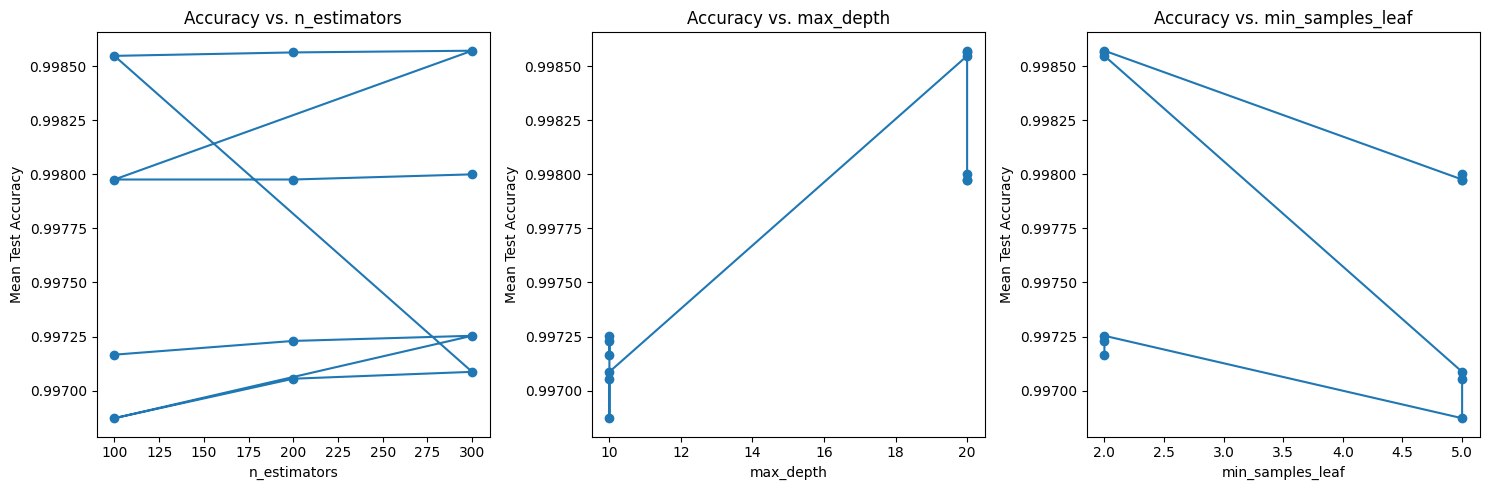
\includegraphics[width=0.9\textwidth]{rfc.png}
  \caption[short]{Random Forest Classifier hyperparameters vs cross validation accuracy.}
\end{figure}

\begin{figure}[h]
  \centering
  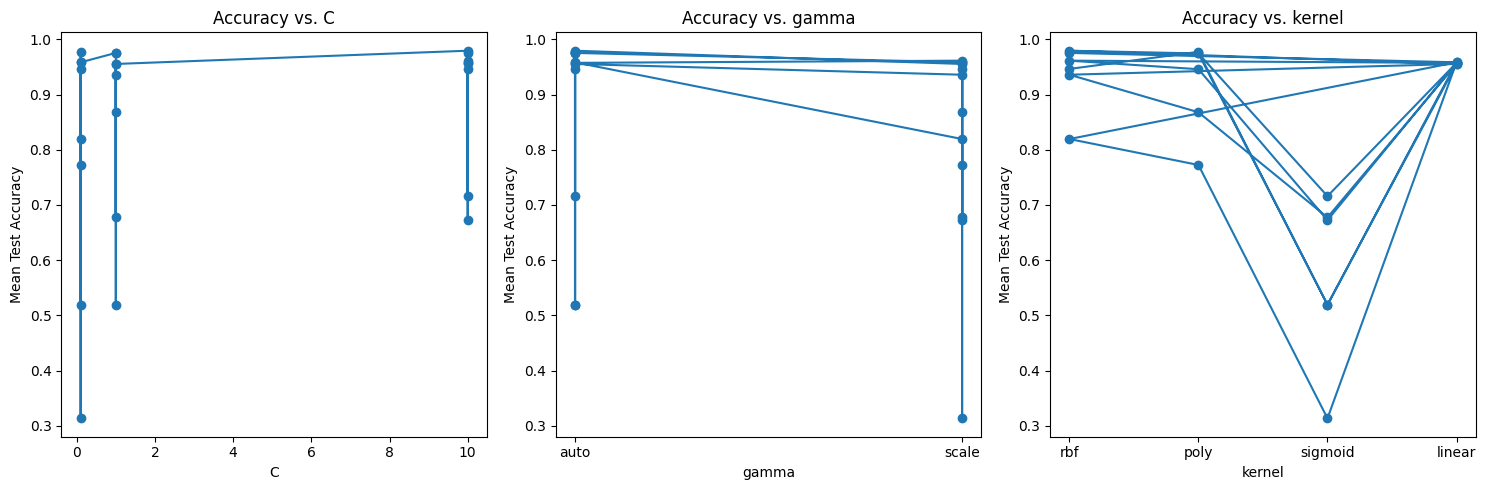
\includegraphics[width=0.9\textwidth]{svm_kernel.png}
  \caption[short]{Kernel SVM hyperparameters vs cross validation accuracy.}
\end{figure}

\section{Results}

The comparitive analysis is done on all 4 different versions of datasets created and using the optimal hyperparametrs for both the models obtained using GridSearchCV. Table \ref{tab:model_performance} presents the performance metrics for each combination.

\begin{table}[htbp]
  \centering
  \setlength{\tabcolsep}{3pt} % reduce padding between columns
  \caption{Model Performance}
  \label{tab:model_performance}
  \begin{tabular}{@{}lcccccccc@{}}
  \toprule
  \textbf{Dataset} & \multicolumn{4}{c}{\textbf{Kernel SVM}} & \multicolumn{4}{c}{\textbf{Random Forest}} \\ 
  \cmidrule(lr){2-5} \cmidrule(lr){6-9}
  & Precision & Recall & F1-Score & Accuracy & Precision & Recall & F1-Score & Accuracy \\
  \midrule
  nsl-kdd & 0.90 & 0.89 & 0.87 & 0.89 & 0.89 & 0.88 & 0.86 & 0.87\\
  nsl-kdd-binary & 0.92 & 0.91 & 0.91 & 0.90 & 0.91 & 0.91 & 0.91 & 0.90\\
  nsl-kdd-fs & 0.89 & 0.89 & 0.87 & 0.88 & 0.88 & 0.88 & 0.86 & 0.87\\
  nsl-kdd-binary-fs & 0.97 & 0.97 & 0.97 & 0.96 & 1.0 & 1.0 & 1.0 & 0.99\\
  \bottomrule
  \end{tabular}
\end{table}

For the NSL-KDD dataset, both Kernel SVM and Random Forest classifiers demonstrated robust performance across all metrics. In particular, the Random Forest classifier achieved high precision, recall, and F1-scores, indicating its effectiveness in binary classification task. However, in the multi-class classification task, where instances are classified into multiple attack types, the Kernel SVM classifier demonstrated competitive performance. Feature selection also seems to have had an impact on the performance of the models which is discussed in the discussions section.


\section{Discussions}


\paragraph{Feature Selection}

The comparison between the original datasets and their feature-selected counterparts reveals a notable improvement in model performance after feature selection. Particularly, in the binary classification task (NSL-KDD-binary), where instances are classified into normal or attack categories, feature selection resulted in higher precision, recall, and F1-scores for both the Kernel SVM and Random Forest classifiers. This improvement indicates that feature selection effectively identified and retained the most relevant features, leading to more accurate and reliable classification results.

Although not explicitly measured in our experiments, it was evident through runtimes that feature selection likely contributes to improved computational efficiency by reducing the dimensionality of the datasets.

While feature selection proved beneficial for binary classification tasks, its impact on multi-class classification tasks, requires further examination. The results suggest that feature selection may have varying effects depending on the complexity of the classification task and the nature of the dataset. 

\paragraph{Kernelized Feature Space}

On the other hand, the competitive performance of the Kernel SVM classifier in multi-class classification tasks may be attributed to its ability to kernelize the data, allowing for the creation of non-linear decision boundaries. By transforming the data into a higher-dimensional space, the Kernel SVM classifier can effectively separate instances belonging to different attack types, leading to accurate classification results. Additionally, the Kernel SVM classifier's margin maximization objective helps in creating decision boundaries that generalize well to unseen data, further enhancing its performance in multi-class classification tasks.


\section*{References}

{
\small
[1] M. Tavallaee, E. Bagheri, W. Lu and A. A. Ghorbani, "A detailed analysis of the KDD CUP 99 data set," 2009 IEEE Symposium on Computational Intelligence for Security and Defense Applications, Ottawa, ON, Canada, 2009, pp. 1-6, doi: 10.1109/CISDA.2009.5356528.

[2] S. S. Wijayanti, E. Utami and A. Yaqin, "Comparison of Kernels on Support Vector Machine (SVM) Methods for Analysis of Cyberbullying," 2022 6th International Conference on Information Technology, Information Systems and Electrical Engineering (ICITISEE), Yogyakarta, Indonesia, 2022, pp. 104-108, doi: 10.1109/ICITISEE57756.2022.10057761.
}

%%%%%%%%%%%%%%%%%%%%%%%%%%%%%%%%%%%%%%%%%%%%%%%%%%%%%%%%%%%%


\end{document}